\documentclass[../mech.tex]{subfiles}
\graphicspath{{\subfix{../figures/}}}
\begin{document}
\chapter{Energy and Momentum of Rotating Systems}
\section{Rotational Kinetic Energy}
The rotational kinetic energy of an object or rigid system is related to the rotational intertia and angular velocity of the rigid system and is given by the equation 
\[ K_R = \frac{1}{2}I\omega^2 \]
The total kinetic energy of a rigid system is the sum of its center of mass and the translational kinetic energy due to the linear motion of the center of mass.
\[ K_{TOT}=K_T+K_R = \frac{1}{2}mv^2+\frac{1}{2}I\omega^2 \]
A rigid system can have rotational kinetic energy while its center of mass is at rest due to the individual points within the rigid system having linear speed, and therefore, kinetic energy.

\begin{example}
    A wheel with rotational inertia $I$ is mounted on a fixed, frictionless axle. The angular speed $\omega$ of the wheel is increased from zero to $\omega_f$ in a time interval $T$.

    What is the average power input to the wheel during this time interval?

    Use power formula: $P=\frac{\Delta k}{t}=\frac{1/2 I\omega_f^2 - \frac{1}{2}I\omega_0^2}{t}$.

    The power is therefore $P=\frac{I\omega_f^2}{2t}$.
\end{example}

\ex Three identical uniform disks, $A$, $B$, and $C$, can each slide along a horizontal surface with negligible friction. Disk $A$ is rotating with angular speed $\omega_A$ while its center of mass remains in place.
Disk $B$ is moving with speed $v_B$ without rotating. Disk $C$ is rotating with the same angular speed $\omega_A$ as Disk $A$ while its center of mass is moving with the same speed $v_B$ as Disk $B$. Which disk has the greatest total kinetic energy?

\ex A solid, uniform disk is spinning about an axis through its center while its center of mass remains at rest. Describe the disk's kinetic energy $K$ with supporting reasoning.

\section{Torque and Work}
A torque can transfer energy into and out of an object or rigid system if the torque is exerted over an angular displacement.
\[ \tau = rF \]
The amount of work done on a rigid system by a torque is related to the magnitude of that torque and the angular displacement through which the rigid system rotates during the interval in which that torque is exerted.
\[ W = \int_{\theta_0}^{\theta} \tau \dd \theta \]
Work done on a rigid system by a given torque can be found from the area under the curve of a graph of the torque as a function of angular position.

\begin{example}
    \begin{center}
        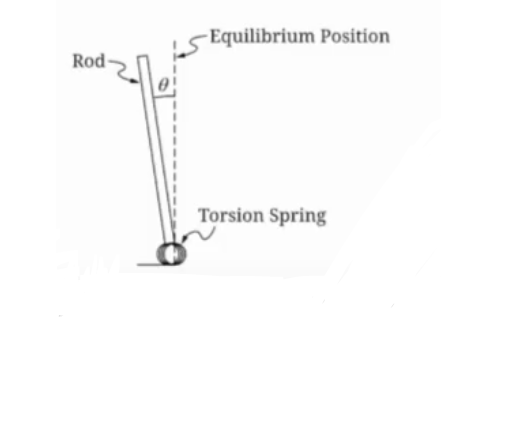
\includegraphics[width=0.5\textwidth]{6.2.PNG}
    \end{center}
    A torsion spring is fixed to the end of rod of rotational inertia $I_R$. The torsion spring is fixed to a horizontal table with negligible friction, as shown in the image. WHen the rod is displaced an angle $\theta$ from equilibrium 
    the torsion spring exerts a restoring torque of magnitude $\tau = 2\kappa \theta^2$, $\kappa$ is a positive constant with appropriate units. After being displaced by an angle $\theta_0$, the rod is released and rotates through its equilibruim position with angular speed 
    $\omega_0$. How much work was done in moving the rod to this position?

    Integrate $2\kappa\theta^2$ from $0$ to $\theta_0$ to get $W=\frac{2\kappa}{3}\theta_0^3$.
\end{example}

\ex \begin{center}
    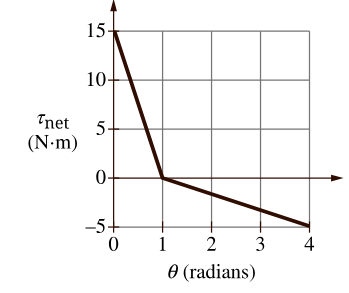
\includegraphics[width=0.5\textwidth]{6.2.2.PNG}
\end{center}
An object can rotate about an axis passing through its center of mass. At $t=0$, the object is spinning in the positive direction and has an initial angular position of zero. The graph represents the net torque $\tau_{net}$ exerted on the object as a function of angular position $\theta$.
What is the total work done on the object and the maximum rotational kinetic energy of the object as it rotates from $0$ radians to $4$ radians?

\ex \begin{center}
    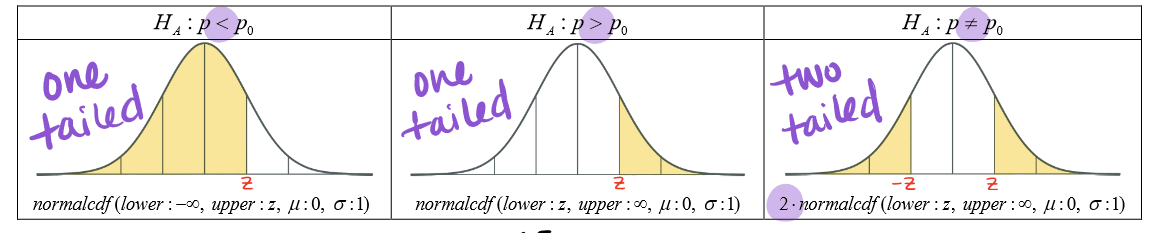
\includegraphics[width=0.5\textwidth]{6.2.1.PNG}
\end{center}
A wheel can rotate about an axis that passes through its center and is perpendicular to the page. THe edge of the wheel is attached to one end of a wire that is connected to a motor, which is fixed in place.
The motor exerts a force on the wire such that the wire exerts a counterclockwise torque of magnitude $\tau_0$ about the center of the wheel when the wheel is at an angular position $\theta_0=0$. As the wheel rotates,
the torque exerted on the wheel changes as a function of $\theta$ that is given by $\tau = \tau_0 e^{-\frac{\theta}{k}}$, where $k$ is a positive constant. If the positive direction for $\theta$ is counterclockwise, how much work is done by the wire 
on the wheel as the wheel rotates from $\theta_0$ to an angular position $\theta_f$?

\section{Angular Momentum and Angular Impulse}
The magnitude of the angular momentum of a rigid system about a specific axis can be described with the equation:
\[ L = I\omega \]
The angular momentum of an object about a given point is 
\[ L = \vec{r}\times \vec{p}=\vec{r}\times m\vec{v}\implies L = mvr\sin \theta \]
Angular impulse is defined as the product of the torque exerted on an object or rigid system at the time interval during which the torque is exerted.
\[ J_{ang}=\int \tau \dd t\]
The magnitude of the change in angular momentum can be described by comparing the magnitudes of the final and initial momenta of the object or rigid system.
\[ \Delta L = \int_{t_0}^{t_1}\tau \dd t\]
A rotational form of the impulse-momentum theorem relates the angular impulse delivered to an object or rigid system and the change in the angular momentum of that object or rigid system.
\[ \tau_{NBT}=\frac{\dd L}{\dd t} \]
\pagebreak
\begin{example}
    A particle of mass $2.0$ kg is moving in the $xy$-plane at a constant speed of $0.80$ m/s in the $+x$-direction along the line $y=4$ m. As the particle travels from $x=-3$ m to $x=+3$ m, what is the magnitude of its angular momentum with respect to the origin?

    $L=mvr = 6.4$ kg$\cdot$m$^2$/s, from the formulas given above.
\end{example}

\ex \begin{center}
    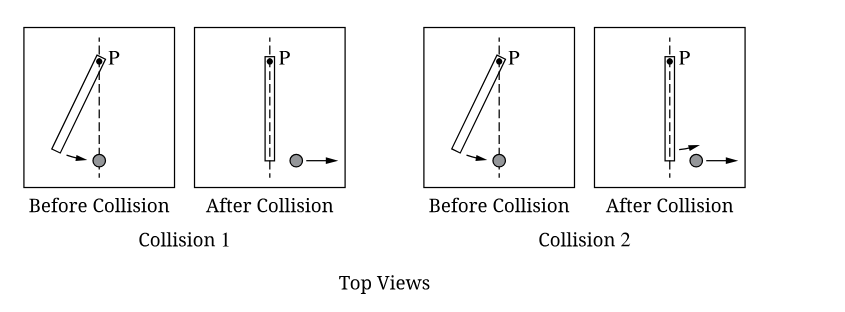
\includegraphics[width=0.5\textwidth]{6.3.PNG}
\end{center}
In the two collisions depicted in the figures, a bar is rotating about a pivot at one end, labeled Point $P$, on top of a horizontal surface before striking a disk that is initially at rest.
The two collisions use the same bar but different disks, where the two disks are the same mass and size but are made of different materials. After each collision, the disk moves to the right at a constant velocity.
After Collision 1, the bar stops rotating. After Collision 2, the bar is still rotating in the same direction, and the disk is moving more slowly than after Collision 1. There is negligible friction between the bar 
and the pivot, between the bar and the surface, and between each disk and the surface. Compare the magnitudes of $J_1$ and $J_2$ of the angular impulse delivered to each disk during their respective collisions, and provide evidence that supports this claim.

\ex \begin{center}
    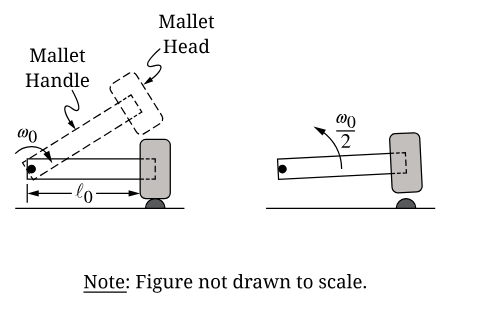
\includegraphics[width=0.5\textwidth]{6.3.1.PNG}
\end{center}
A mallet rotates about a pivot near one end of its handle and is moving clockwise with an angular speed $\omega_0$ as it strikes a small, stationary rubber bumper, as shown in the figure. Immediately after the impact, the mallet is rotating counterclockwise about the pivot with an angular speed 
$\frac{\omega_0}{2}$. The handle of the mallet has length $l_0$, mass $m_0$, and rotational inertia $I_0 = \frac{1}{3}m_0l_0^2$ about the pivot. The head of the mallet is small compared to the length of the handle, has the same mass $m_0$ as the handle, and is located a distance 
$l_0$ from the pivot. If the mallet is in contact with the bumper for an amount of time $\Delta t$, what is the magnitude of the average force that the mallet exerts on the rubber bumper during the contact time?

\section{Conservation of Angular Momentum}
The total angular momentum of a system about a rotational axis is the sum of the angular momenta of the system's constituent parts about that axis of rotation.

Any change to a system's angular momentum must be due to an interaction between the system and its surroundings.

Angular momentum is conserved in all interactions.

If the net external torque is exerted on a selected object or rigid system is:
\begin{itemize}
    \item Zero: the total angular momentum is constant 
    \item Nonzero: angular momentum is transferred between the system and the environment 
\end{itemize}

\begin{example}
    A circular platform has a radius $R$ and rotational inertia $I$. The platform rotates about a fixed pivot at its center with negligible friction and an initial angular velocity $\omega$.
    A child of mass $m$ rungs tangentially with speed $v$ and jumps on the outer edge of the platform. When the child is standing on the outer edge of the platform, what is the system's new angular velocity?

    We have $L_{c_i}+L_{p_i}=L_T$, so we get $mvr+I\omega = (I_c+I_p)\omega_f$.

    Solving for $\omega_f$ gives $\frac{mvr+I\omega}{I+mr^2}$
\end{example}

\ex \begin{center}
    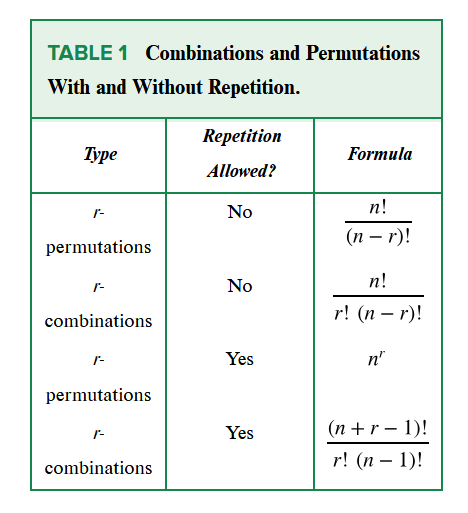
\includegraphics[width=0.5\textwidth]{6.4.PNG}
\end{center}
A small disk can move on a horizontal surface with negligible friction. The disk is attached to a string that passes through a small hole in the surface and is held in place at the other end, under the surface.
Initially, the disk is moving in a circle of radius $0.10$ m about the hole with an angular speed of $4.0$ rad/s. The bottom end of the string is then raised upward so that the disk travels in a new circle of radius $0.20$ m. What is the angular speed of the disk at the new radius?

\ex \begin{center}
    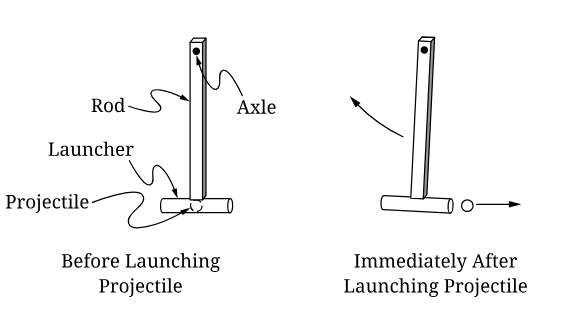
\includegraphics[width=0.5\textwidth]{6.4.1.PNG}
\end{center}
A projectile launcher is attached to one end of a rod, as shown in the figure. The other end of the rod can pivot freely about an axle with negligible friction. Initially, the rod and launcher, with a projectile inside, are all at rest. The projectile is then launched to the right, 
causing the rod and launcher to recoil in the clockwise direction. Immediately after the projectile is launched, what is true regarding both the angular momenta of the rod-launcher system and the projectile, and the kinetic energies of the rod-launcher system and the projectile? Angular momentum is to be taken about the axle.

\section{Rolling}
The total kinetic energy of a system is the sum of the system's translational and rotational kinetic energies.

While rolling without slipping, the translational motion of a system's center of mass is related to the rotational motion of the system itself with the following equations:
\[ x_{cm}=r\theta \]
\[ v_{cm} = r\omega \]
\[ a_{cm}=r\alpha \]
Rolling without slipping implies that the frictional force does not dissipate any energy from the system.

If the rolling object is slipping, the force of kinetic friction moves with respect to the surface, so the force of kinetic friction will dissipate energy from the system.

\begin{example}
    A sphere of mass $M$, radius $r$, and rotational inertia $I$ is released from rest at the top of an inclined plane of height $h$. If the plane has friction so that the sphere rolls without slipping, whta is the speed $v_{cm}$ of the center of mass at the bottom of the incline?

    The inertia is $\frac{2}{5}mr^2$.

    We know that the there is no kinetic energy initially and all the energy is kinetic at the bottom of the plane, so $U_i=K_f$.

    Plugging numbers gives us $mgh=K_T+K_R=\frac{1}{2}mv^2+\frac{1}{2}I\omega^2$.

    When we solve for $v$, we get $\sqrt{\frac{10}{7}gh}=v$.
\end{example}

\ex \begin{center}
    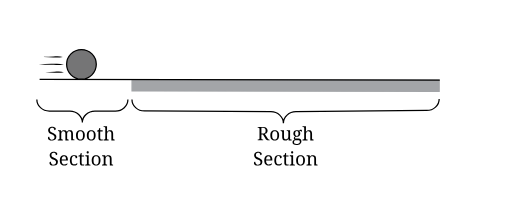
\includegraphics[width=0.5\textwidth]{6.5.PNG}
\end{center}
A solid sphere is initially moving at a constant speed $v_0$ on a horizontal surface, as shown in the figure. At first, the sphere is sliding without rotating and moves with negligible friction on a smooth section of the surface. The sphere then reaches a rough section of the surface 
where the coefficient of kinetic friction is $\mu_k$. Sometime later, the sphere is rolling without slipping on the rough section. The sphere has a mass $m_S$, a radius $r_S$, and a rotational inertia about its center $I_S=\frac{2}{5}m_Sr_S^2$. What is the final angular speed of the sphere?

\ex \begin{center}
    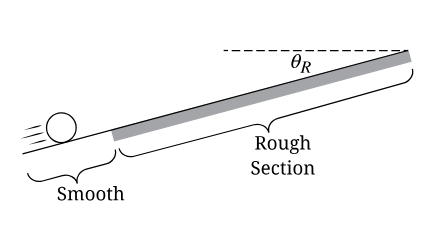
\includegraphics[width=0.5\textwidth]{6.5.1.PNG}
\end{center}
A hollow cylinder is initially sliding without rotating up a smooth section of a ramp that makes an angle $\theta_R$ with the horizontal, as shown in the figure. The cylinder then reaches a rouch section of the ramp where the coefficient of kinetic friction between the cylinder and the ramp is $\mu_k$. 
The cylinder, which has mass $m_C$, radius $r_C$, and rotational inertia about its center of $I_C=m_Cr_C^2$, starts to rotate while slipping on the rough section of the ramp. When the cylinder is rolling upward while slipping on the rough section, what is the magnitude $a$ of the cylinder's translational acceleration in terms of the magnitude $\alpha$ of its angular acceleration and the given quantities?

\section{Motion of Orbiting Satellites}
In a system consisting only of a massive central object and an orbiting satellite with mass that is negligible to the central object's mass, the motion of the central object itself is negligible.

The motion of satellites in orbits is constrained by conservation laws.
\begin{itemize}
    \item In circular orbits, mechanical energy, potential energy, kinetic energy, and angular momentum are conserved.
    \item In elliptical orbits, mechanical energy and angular momentum are conserved, but potential and kinetic energies are not.
    \item The gravitational PE is defined to be zero when a satellite is an infinite distance from the central object.
\end{itemize}
The total energy of a system with a central object and an orbiting satellite can be written in terms of GPE.

The escape velocity of a satellite is the satellite's velocity such that the ME of the satellite-central object system is equal to zero.

\begin{example}
    A rocket of mass $m$ is launched from the surface of Earth with an initial speed equal to one-half the escape speed. The mass and the radius of Earth are $6.0\times 10^{24}$ kg and $6.4\times 10^6$ m, respectively. What is the maximum altitude achieved by the rocket? Assume air resistance is negligible.

    Start with $V_E = \sqrt{\frac{2GM}{R}}$ and plug this into $K=\frac{1}{2}mv^2$ to get $\Delta K = \frac{1}{4}\frac{GMm}R$.

    From this, we know that $\Delta U = U_f-U_i$.

    This gives us $\frac{1}{4}\frac{GMm}{R}=-\frac{GMm}{R+h}+\frac{GMm}{R}$.

    From this, solving for $h$ gives $h=\frac{1}{5}R$.
\end{example}

\ex Two satellies with the same mass, Satellite $X$ and Satllite $Y$, are in different circular orbits around a planet. Satellite $Y$ orbits with twice the speed of Satllite $X$. If $U_X$ is the gravitational potential energy of the Satellite $X$-planet system, what is the gravitational potential energy of the Satellite $Y$-planet system?

\ex \begin{center}
    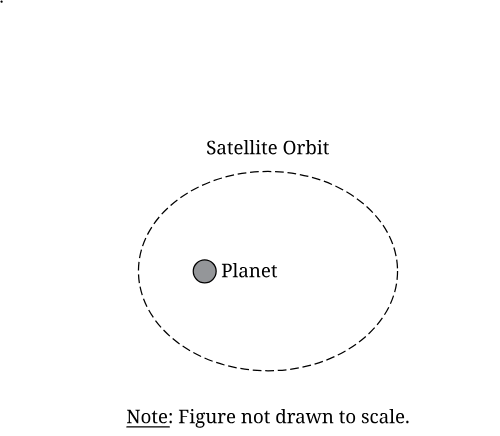
\includegraphics[width=0.5\textwidth]{6.6.PNG}
\end{center}
A satellite is in an elliptical orbit around a planet, as shown in the figure. Why does the satellite's kinetic energy change as it orbits the planet?

\end{document}